% Appendix version after 9-page restructure (step 2)
% =====================================================================
% Why rank-1 damping fails: the self-stabilization cap -- theory appendix
% Extends Damian et al. (2023). The 2/eta threshold is a self-stabilization
% CAP enforced by the period-2 EoS oscillation, not a controllable floor.
% Rank-1 damping either fails to engage (cap intact -> pins at 2/eta) or
% removes the cap (upward escape above 2/eta). Neither achieves descent
% below the threshold.
% The same fixed-point algebra at gamma < 0 (rank-1 AMPLIFICATION) moves the
% equilibrium BELOW 2/eta -- confirmed experimentally -- so the dichotomy is
% attenuation-vs-amplification, not local-vs-global. The alternative
% "spectral migration" reading is ruled out by the rank-k and multi-sharp
% experiments; the re-acquire diagnostic that motivated it reduces to the
% free-v case (see (b) below).
% =====================================================================

This appendix develops the reduced-model account behind the full-batch
experiments. Within the two-dimensional self-stabilization reduction, damping
the top-gradient component does not create a sub-threshold sign-flip orbit;
reversing the sign moves the corresponding orbit below $2/\eta$. Thus the
relevant distinction in this reduction is attenuation versus amplification
rather than local versus global action. The formal result concerns orbit
location, while the accompanying experiments test several alternative
explanations for the observed network trajectories, including spectral
migration and sensing failure. Section~\ref{app:mig-struct} states the
account and its direct tests, Section~\ref{app:mig-dyn} derives the reduced
recurrence, Section~\ref{app:mig-formal} states the formal orbit-location
lemma and its stability limitations, and the remaining controls
(\S\ref{app:two-controls}) delimit which parts of the account extend beyond
the reduction.

\subsection{The self-stabilization cap, and why rank-1 damping has no sub-threshold sign-flip orbit}
\label{app:mig-struct}

\begin{claim}[reduced-model interpretation; informal]
\label{clm:rank1}
The EoS threshold $2/\eta$ is a self-stabilization \emph{cap}: the period-2
oscillation of the iterate along the top eigenvector $u_{1}$ generates, via the
cubic identity $\nabla S=\nabla^{3}L(u_{1},u_{1})$ of
\citet{damian2023selfstab}, a restoring force that balances progressive
sharpening and pins $S=\lmax$ at $2/\eta$. In this reduction, a rank-1 gradient edit that \emph{damps}
the gradient component along an estimate $\hat v$ of $u_{1}$ creates no
sub-threshold sign-flip orbit; empirically it lands in one of two
regimes, neither of which descends below the threshold:
\begin{itemize}
  \item \emph{Imperfect damping} ($\hat v$ lags $u_{1}$, e.g.\ the free
        $\hat v=\Delta\theta_{t-1}/\|\cdot\|$): the parallel-gradient
        cancellation is incomplete, the period-2 oscillation persists, and
        self-stabilization caps $\lmax$ at $2/\eta$.
  \item \emph{Accurate damping} ($\hat v\approx u_{1}$ via power iteration):
        the directional rescaling is applied to the correct sharp direction.
        At the original boundary $\lambda=2/\eta$, the effective top-direction
        step lies inside its previous sign-flip boundary, weakening the
        oscillatory balance that supported the original cap. For fixed $d$,
        progressive sharpening can then continue until the sign-flip condition
        is re-established at $\lambda=2d/\eta$; under adaptive self-gating,
        the reduced model does not determine a finite raw-sharpness endpoint.
        Thus accurate damping releases the original $2/\eta$ cap rather than
        eliminating sign-flip dynamics altogether.
\end{itemize}
Within the reduced sign-flip account, a sub-threshold orbit requires the
amplifying sign. SAM provides a separate global benchmark whose first-order
correction has this sign along positive-curvature directions; the
``spectral migration'' alternative, that damping the current top direction
causes another eigendirection to become dominant, is \emph{not} what
the experiments show.
\end{claim}

This matches \emph{all} empirical controls, including the following
controls, several designed specifically to probe migration:
(a) the free-$\hat v$ optimizer locks at $\lmax^{\mathrm{final}}=40.12\pm0.12=2/\eta$
(regime (i): the lagged $\hat v$ preserves the oscillation, so the cap holds);
(b) the ``re-acquire the correct $v_{\mathrm{top}}$'' variant does \emph{not}
test accurate $v_{\mathrm{top}}$ every step: the refreshed vector is overwritten
by the next step's free $\Delta\theta$ at the end of each step, so it reduces to
variant (a) save one step. Its $40.019\pm0.002$ therefore supports regime (i).
The accurate-$v_{\mathrm{top}}$ test is the rank-k sweep below;
(c) the free-$\hat v$ diagnostic $\hat\lambda=\hat v^{\!\top}\!H\hat v$
\emph{does} collapse to $\sim\!10^{-4}$ while true $\lmax$ stays at $40$, but
this is a \emph{$\hat v$-tracking failure}, not a migration signature: the
trajectory's only sharp axis is $u_{1}$, and once the lagged $\hat v$ rotates
out of it (as the active window changes the update direction) $\hat\lambda$
measures a subdominant axis: a measurement artifact, not sharpness flow;
(d) SAM escapes ($21.35\pm0.04<2/\eta$) because its perturbation
$\varepsilon=\rho\mathbf{g}/\|\mathbf{g}\|$ acts in \emph{every} direction
simultaneously, so there is no eigenvector whose cap is selectively removed;
the matched-step X-SAM projector ablation (Appendix~\ref{app:xsam}, $n{=}10$) shows the rank-1 half
of an eigenvector-aware SAM fires every step yet has no detectable effect on
$\lmax$ at this power (paired $\Delta{=}+0.62$, 95\% CI $[-0.61,+1.85]$;
reductions beyond ${\sim}0.61$ reference-sharpness units are excluded).

\paragraph{The rank-k sweep is inconsistent with migration on the 1-D-sharp landscape.}
Replacing the free $\hat v$ by \emph{accurate} warm-started power iteration of
the top-$k$ eigenvectors (block power iteration $+$ modified Gram--Schmidt) and
damping all $k$ components, the optimizer enters regime (ii): with $k\!=\!1$ the edit accurately
rescales the only sharp direction, releasing the original $2/\eta$ cap; raw
sharpness then escapes upward to $261.8\pm5.4$ (lower loss $0.090$ than GD's
$0.111$, but \emph{sharper}, opposite to the control objective). Crucially
$k\!=\!1,2,5,10$ are bit-identical: the spectrum is $1$-D sharp
($\lambda_{1}\!=\!261.8\!\pm\!5.4$, $\lambda_{2}\!\approx\!0.6$; over two
orders of magnitude), so there is \emph{nowhere for sharpness to migrate to}; damping
more directions changes nothing. The $k$-invariance is predicted by the
cap-removal mechanism (one accurately damped direction suffices to release
the cap on the only oscillating direction) and is inconsistent with migration (which predicts more damping
$\Rightarrow$ lower $\lmax$).

\paragraph{ResNet-18 rank-$k$ is an outcome-level null, not an engagement
failure.}
One might worry the MLP $k$-invariance above merely confirms the $1$-D-sharp
geometry rather than telling against migration. The ResNet-18 rank-$k$ sweep
(heavy-tailed spectrum, not $1$-D sharp) addresses this worry only
partially: as established in \S\ref{sub:scale}, with deterministic
ARPACK-based sensing the edits fire as designed (verified engagement at
every tested $k\le20$), yet no damping arm produces a statistically resolved
reduction of the reference $\lmax$ relative to SGD at this power: the null
is at the
outcome level, not the engagement level. (An earlier power-iteration
false-convergence had initially left the clamped optimizer effectively
dormant; after the sensing correction, the absence of a statistically
resolved reduction persists at this operating point, so the earlier
dormancy does not explain the observed null.) The sweep therefore contributes the scale reproduction of
the \emph{ordering} (no descent below the SGD band at any attenuating $k$; only full
SAM escapes), not an independent test of migration; the evidence against
migration rests on the MLP multi-sharp test below.

\paragraph{The multi-sharp-landscape test is inconsistent with migration where it could
plausibly act.}
As established in \S\ref{sub:migration}: on a constructed multi-sharp landscape
(two directions pinned at $2/\eta$), damping only $u_{1}$ lets $u_{1}$
escape upward while $\lambda_{2}$ stays pinned (there is no flow from $u_{1}$
to $u_{2}$) and, unlike the $1$-D case, $k$ \emph{does} matter, each direction
whose cap is removed escaping independently and revealing the
\emph{per-direction} structure of the cap. The multi-sharp construction is
therefore used as a stress test of the per-direction account; we do not infer
the typical dimensionality of the sharp Hessian subspace from
trajectory-PCA dimensionality. Across both landscapes the verdict is identical: no descent below the threshold, and
no migration.

The non-separable multi-sharp experiment provides evidence consistent with
per-direction capping in one constructed landscape; it does not establish
general multi-eigenvalue decoupling: the regime
\citet{damian2023selfstab} flag as open (\S8.2).

\subsection{Supporting heuristic: the damped self-stabilization dynamics}
\label{app:mig-dyn}

The cap-removal account is the dynamics-level avatar of
\citet{damian2023selfstab}. Let $S(\theta)=\lmax(H)$ with simple top pair
$(\lambda_{1},u_{1})$, $x_{t}$ the iterate's displacement along $u_{1}$,
$y_{t}=S-2/\eta$, $\alpha_{\mathrm{ps}}=-\nabla L\!\cdot\!\nabla S>0$ the progressive-sharpening
coefficient (their Def.~2), and $\beta=\|\nabla S\|^{2}$. Their keystone identity
$\nabla S=\nabla^{3}L(u_{1},u_{1})$ (their Lemma~2) yields the 2-D recurrence
(their eq.~3)
\begin{equation}
x_{t+1}=-(1+\eta y_{t})\,x_{t},\qquad
y_{t+1}=y_{t}+\eta\!\left(\alpha_{\mathrm{ps}}-\tfrac{\beta}{2}x_{t}^{2}\right),
\label{eq:damian}
\end{equation}
whose period-2 fixed point $|x_{t}|\!\to\!\delta=\sqrt{2\alpha_{\mathrm{ps}}/\beta}$ pins
$S=\lambda_{1}\approx 2/\eta$ by balancing progressive sharpening $\alpha_{\mathrm{ps}}$
against the cubic restoring force $\tfrac{\beta}{2}x^{2}$ generated by the
iterate moving along $u_{1}$. This is the self-stabilization \emph{cap} of
Claim~\ref{clm:rank1}: the oscillation $x_{t}$ is what holds $\lmax$ at $2/\eta$.

\paragraph{Effect of rank-1 damping (heuristic).}
The optimizer edits the gradient to $g'=g-\gamma(g^{\top}\hat v)\hat v$ with
$\gamma=1-1/d\in(0,1)$, $d=\max(\hat\lambda/(2/\eta),1)$. Taking $\hat v\approx u_{1}$ and treating $d$ as
fixed over a local window, the displacement along $u_{1}$ evolves as
\begin{equation}
x_{t+1}=\bigl(1-(1-\gamma)\eta\lambda_{1}\bigr)x_{t}
       =\bigl(-1+2\gamma-(1-\gamma)\eta y_{t}\bigr)x_{t},
\label{eq:damped-x}
\end{equation}
while the restoring-force recurrence in $y$ retains the form
$y_{t+1}=y_{t}+\eta(\alpha_{\mathrm{ps}}-\tfrac{\beta}{2}x_{t}^{2})$: the edited
optimizer's first-order sharpness increment is
$-\eta\langle\nabla S,g'\rangle=\eta\alpha_{\mathrm{ps}}+\eta\gamma(g^{\top}u_{1})(u_{1}^{\top}\nabla S)$,
and expanding $g^{\top}u_{1}=\lambda_{1}x+\tfrac12(u_{1}^{\top}\nabla S)x^{2}+O(x^{3})$
(the same along-axis truncation that yields \eqref{eq:damped-x}) decomposes the
correction into an $x$-odd ripple of zero mean over the sign-flip cycle (the
class of terms the \emph{undamped} reduction of \citet{damian2023selfstab}
already discards in freezing $\alpha_{\mathrm{ps}}$ to a constant) and an
$x$-even remnant $\tfrac{\gamma}{2}(u_{1}^{\top}\nabla S)^{2}x^{2}$ that only
renormalizes the amplitude-setting coefficient $\beta$. Since the orbit
\emph{location} $y^{*}$ follows from the $x$-recurrence alone, neither piece
moves $\lambda^{*}=2d/\eta$. Solving
\eqref{eq:damped-x} for the period-2 fixed point ($x_{t+1}=-x_{t}$) gives an
equilibrium excess
\begin{equation}
y^{*}=\tfrac{2\gamma}{(1-\gamma)\eta},
\qquad\tfrac{\partial y^{*}}{\partial\gamma}=\tfrac{2}{(1-\gamma)^{2}\eta}>0
\ \ \text{for all }\gamma<1:
\label{eq:ystar}
\end{equation}
 the sign-flip orbit location is \emph{strictly increasing in the sign of the edit}.
Damping ($\gamma\in(0,1)$) gives $y^{*}>0$; the sign-flipped
\emph{amplification} edit ($\gamma=-\alpha<0$, i.e.\
$g'=g+\alpha(g^{\top}\hat v)\hat v$) gives
$y^{*}=-\tfrac{2\alpha}{(1+\alpha)\eta}<0$ with equilibrium sharpness
$\lambda^{*}=2/((1+\alpha)\eta)<2/\eta$: \emph{descent below the threshold by a rank-1
single-direction edit} (Corollary~\ref{cor:amplify}). The reduction thus
does not support a local-vs-global dichotomy; it supports an
\emph{attenuation-vs-amplification} one, of which SAM's global perturbation
is one first-order instance of the amplifying sign
(Remark~\ref{cor:sam}).

\paragraph{What the heuristic predicts, and what it does not.}
The content to keep is the \emph{sign} of the prediction, not a magnitude:
$y^{*}>0$ says accurate damping moves the sign-flip orbit location
\emph{past} $2/\eta$
(upward, opposite to the control goal), and this is what the
accurate-$v_{\mathrm{top}}$ experiment confirms (an upward escape on the 1-D
landscape, $\sim\!65$ on the multi-sharp one). Symmetrically, $y^{*}<0$ at
$\gamma<0$ says amplification moves the sign-flip orbit location
\emph{below} $2/\eta$,
and this is what the sign-flip control confirms
(\S\ref{sub:amp}): late-window equilibria
$30.1\!\pm\!0.5\,/\,22.5\!\pm\!1.3\,/\,14.3\!\pm\!2.7$ at
$\alpha\!=\!0.25\,/\,0.5\,/\,1$ ($n{=}5$), all strictly below $2/\eta\!=\!40$
and monotone in $\alpha$, though each sits \emph{below} the naive
fixed-point value $\lambda^{*}\!=\!2/((1{+}\alpha)\eta)$
($32\,/\,26.7\,/\,20$); the magnitude disclaimer below applies
symmetrically to both signs. Neither sign predicts the escape magnitude: under the self-gating rule $d=\hat\lambda/(2/\eta)$,
$\gamma=1-1/d$, the fixed-point condition $y^{*}=2\gamma/((1-\gamma)\eta)$ is
satisfied for \emph{every} $\lambda_{1}>2/\eta$ (substituting $\gamma$ reduces
it to the identity $y^{*}=y$); the magnitude is set by where unopposed
progressive sharpening equilibrates, a quantity the 2-D reduction does not fix.
The free-lagged-$\hat v$ variant, by contrast, falls \emph{outside} this
derivation: once the active window changes the update direction, $\hat
v\not\approx u_{1}$, so $\hat\lambda=\hat v^{\!\top}\!H\hat v$ reads a
subdominant axis and the self-gating $d$ is set by the wrong curvature; the
$u_{1}$-oscillation that \eqref{eq:damped-x} targets is essentially untouched,
the cap holds, and $\lmax\approx 2/\eta$. The two regimes of
Claim~\ref{clm:rank1} are thus two cases of \emph{whether the derivation's
$\hat v\approx u_{1}$ premise holds}: accurate $\hat v$ enters the $y^{*}>0$
regime (cap removed, upward escape); lagged $\hat v$ never engages the $u_{1}$
axis and the cap is never at risk.

\paragraph{Scope of the reduced-model interpretation.} Claim~\ref{clm:rank1} is a
reduced-model interpretation, not a trajectory theorem. Its multi-direction
premise is empirically supported in the constructed multi-sharp test but
remains theoretically open in general (\textbf{G1}). The reduced-dynamics heuristic
\eqref{eq:damian}--\eqref{eq:damped-x} postulates per-direction decoupling,
which is the multi-eigenvalue extension \citet{damian2023selfstab} explicitly
defer to future work (\S8.2), and is formally singular at the rotation instant
$\lambda_{1}=\lambda_{j^{*}}$ (their Lemma~2 needs $\lmax$ simple); there one
works with the individual gradients $\nabla\lambda_{i}$ rather than $\nabla S$.
We tested the ``spectral migration'' alternative (sharpness flowing to an
undamped direction) directly on a multi-sharp landscape and it did not manifest
($\lambda_{2}$ stayed pinned while $u_{1}$ escaped); we therefore present
migration only as a hypothesis that these tests do not support, and the cap-removal
account as the one the data support. The core algebraic content of
Claim~\ref{clm:rank1} (that no period-2 fixed point of the damped recurrence
has $y\leq0$) is made rigorous, with a stability analysis, in
Lemma~\ref{prop:boundary} below; the gaps that remain before a
full trajectory theorem are itemized there (\textbf{G1}--\textbf{G5}). The
division of labor is deliberate and should be read as such:
 Lemma~\ref{prop:boundary} is a \emph{reduced-map
statement} (it constrains sign-flip period-2 orbits of the 2-D recurrence under
\textbf{A1}--\textbf{A3}, not trajectories of the network) and every
mechanistic statement that reaches beyond that reduction (optimizers with sensed
$\hat v$, non-sign-flip transients, the stochastic regime) is carried by the
interventional experiments of \S\ref{sec:control}--\S\ref{sub:scale}, not by the
lemma.

\subsection{Formal lemma: no flat sign-flip orbit under rank-1 damping
(2-D reduction)}
\label{app:mig-formal}

We upgrade the heuristic above to a formal statement on Damian et al.'s 2-D
recurrence. The addition over \eqref{eq:damped-x}--\eqref{eq:damian} is a
\emph{conditional $y$-contraction} analysis: not only is the period-2 fixed
point at $y^{*}>0$, the two-step $y$-direction multiplier (conditional on $x$
remaining on the period-2 orbit) is contractive under a checkable condition. We
label this \emph{conditional $y$-contraction}, not stability: the full 2-D map
is normally repelling (Remark~\ref{rem:jacobian}), and orbit stability would
additionally require the higher-order $|x|$-bounding of gap~\textbf{G4}.

\paragraph{Setup.}
Recall $S(\theta)=\lmax(H)$, $y=S-2/\eta$, the top pair $(\lambda_{1},u_{1})$,
$x_{t}$ the iterate's displacement along $u_{1}$,
$\alpha_{\mathrm{ps}}=-\nabla L\!\cdot\!\nabla S>0$
and $\beta=\|\nabla S\|^{2}>0$. The $y$-recurrence is
\begin{equation}\label{eq:Damian-y}
y_{t+1}=y_{t}+\eta\!\left(\alpha_{\mathrm{ps}}-\tfrac{\beta}{2}x_{t}^{2}\right),
\end{equation}
and the rank-1-damped $x$-recurrence (gradient edit
$g\mapsto g-\gamma(g^{\top}\hat v)\hat v$, $\gamma=1-1/d\in(0,1)$, $\hat v=u_{1}$)
is
\begin{equation}\label{eq:damped-x-formal}
x_{t+1}=\bigl(-1+2\gamma-(1-\gamma)\eta y_{t}\bigr)x_{t}.
\end{equation}
Let $F$ be the 2-D map defined by \eqref{eq:damped-x-formal}--\eqref{eq:Damian-y}.

\begin{assumption}[\textbf{A1}: positive isolated top pair]
Along the analysis window, $\lambda_{1}(\theta)\geq m>0$ and
$\lambda_{1}(\theta)-\lambda_{2}(\theta)\geq\Delta>0$, so the top eigendirection
and $\nabla S$ are well defined \citep{damian2023selfstab}.
\end{assumption}

\begin{assumption}[\textbf{A2}: window-fixed edit strength]
The edit strength is constant over the analysis window: damping
$\gamma\in(0,1)$ (it evolves on $O(1/\eta)$ steps; $x$-dynamics is
$O(1)$); the sign-flipped amplifying edit $\gamma=-\alpha<0$ is treated
under the same window assumption in Corollary~\ref{cor:amplify}.
\end{assumption}

\begin{assumption}[\textbf{A3}: accurate sensing]
$\hat v=u_{1}$ (an idealization; within the reduced top-direction equation,
an angular sensing error $\varphi$ reduces the effective damping to
$\gamma\cos^{2}\varphi$, cf.\ gap~\textbf{G5}; off-axis effects lie outside
the reduction).
\end{assumption}

\begin{quote}
\emph{Lemma 1, restated in detailed form.} Under \textbf{A1}--\textbf{A3}, for the damped map $F$ with
$\alpha_{\mathrm{ps}},\beta,\eta>0$, $\gamma\in(0,1)$:
\begin{itemize}
  \item[\textbf{(a)}] \emph{Algebraic.} Every \emph{sign-flip} period-2 fixed
        point of $F$, one with $F(x_{*},y_{*})=(-x_{*},y_{*})$ and
        $|x_{*}|>0$, satisfies $y^{*}=\tfrac{2\gamma}{(1-\gamma)\eta}>0$ and
        $|x_{*}|=\sqrt{2\alpha_{\mathrm{ps}}/\beta}$. In particular, \emph{no sign-flip
        period-2 orbit has $y^{*}\leq0$}. (The map $F^{2}$ admits additional
        non-sign-flip period-2 orbits for $\kappa>4$, with $y$ alternating
        between two negative values; these require $y<-\tfrac{2}{\eta}$, i.e.\
        $S=\lmax<0$, contradicting \textbf{A1} ($\lambda_{1}\geq m>0$). We exclude them on
        these \emph{physicality} grounds, not on stability grounds: the
        sign-flip orbit the lemma analyzes is \emph{itself} a full-map
        repeller (Remark~\ref{rem:jacobian}), so instability cannot be the
        criterion that separates the two orbit families.)
  \item[\textbf{(b)}] \emph{Conditional $y$-contraction (not stability).} With $\kappa:=2(1-\gamma)\eta^{2}\alpha_{\mathrm{ps}}>0$,
        the two-step $y$-direction multiplier \emph{conditional on $x$ remaining
        on the period-2 orbit} is $\mu_{y}=1-\kappa$, satisfying $|\mu_{y}|<1$
        iff $(1-\gamma)\eta^{2}\alpha_{\mathrm{ps}}<1$. This is a \emph{conditional
        $y$-contraction}, a contraction of the slow $y$-direction on the
        invariant graph $x\in\{\pm x_{*}\}$, not an orbit-stability result: the
        full 2-D map is normally repelling (Remark~\ref{rem:jacobian}), and orbit
        stability additionally requires the higher-order $|x|$-bounding of
        gap~\textbf{G4}, which the 2-D reduction cannot supply.
\end{itemize}
\end{quote}

\begin{proof}
\emph{(a)} Impose the period-2 ansatz $x_{t+1}=-x_{t}$ in
\eqref{eq:damped-x-formal}: $-x_{*}=(-1+2\gamma-(1-\gamma)\eta y^{*})x_{*}$, so
$y^{*}=\tfrac{2\gamma}{(1-\gamma)\eta}>0$ (positive since $\gamma\in(0,1)$).
Monotonicity $\partial y^{*}/\partial\gamma=2/((1-\gamma)^{2}\eta)>0$: stronger
damping strictly raises the sign-flip orbit location. The $y$-recurrence
\eqref{eq:Damian-y} on the orbit ($y$ invariant over two steps) forces the
increment to vanish, giving $|x_{*}|=\sqrt{2\alpha_{\mathrm{ps}}/\beta}$, identical to the
undamped amplitude $\delta=\sqrt{2\alpha_{\mathrm{ps}}/\beta}$ \citep{damian2023selfstab}:
damping relocates $y^{*}$ but not the orbit amplitude.

\emph{(b)} Singular-perturbation (slow--fast) analysis: $y$ is slow (per-step
drift $O(\eta)$), $x$ is fast (per-step sign-flip). Perturb $y\to y^{*}+\varepsilon$
keeping $x$ on the fast manifold. Writing $m(y):=-1+2\gamma-(1-\gamma)\eta y$
(so $m(y^{*})=-1$): step~1 gives $x_{1}=(-1-(1-\gamma)\eta\varepsilon)x_{*}$ and
$y_{1}=y^{*}+\varepsilon$ (the $y$-increment vanishes by
$|x_{*}|=\sqrt{2\alpha_{\mathrm{ps}}/\beta}$); step~2 then yields, using
$x_{1}^{2}=(1+2(1-\gamma)\eta\varepsilon)x_{*}^{2}+O(\varepsilon^{2})$ and
$\beta x_{*}^{2}=2\alpha_{\mathrm{ps}}$,
\begin{equation}
y_{2}=y^{*}+\varepsilon-\underbrace{2(1-\gamma)\eta^{2}\alpha_{\mathrm{ps}}}_{=:\,\kappa}\,\varepsilon
+O(\varepsilon^{2})=y^{*}+(1-\kappa)\,\varepsilon+O(\varepsilon^{2}).
\label{eq:mustar}
\end{equation}
Thus $\mu_{y}=1-\kappa$, conditionally $y$-contractive (on the invariant graph
$x\in\{\pm x_{*}\}$) iff $|1-\kappa|<1\iff
(1-\gamma)\eta^{2}\alpha_{\mathrm{ps}}<1$.
\end{proof}

\begin{remark}[scope of stability]
\label{rem:scope}
The orbit above is repelling for the full 2-D Jacobian
(Remark~\ref{rem:jacobian} below): a complete stability argument would
require the higher-order $|x|$-bounding of gap~\textbf{G4}, which the
2-D reduction cannot supply, and we leave this open. The result is
used as an orbit-location prediction only.
\end{remark}

\begin{remark}[degenerate and unstable fixed points outside scope]
\label{rem:degenerate}
$F$ also has a degenerate period-1 fixed point at $y=-2/\eta$ (i.e.\ $S=0$,
$\lambda_{1}=0$), outside the EoS regime $\lambda_{1}\approx2/\eta$. When
$(1-\gamma)\eta^{2}\alpha_{\mathrm{ps}}\ge1$ (i.e.\ $\kappa\ge2$) the conditional
$y$-multiplier $|\mu_{y}|\ge1$ and the equilibrium loses even conditional
stability, plausibly the route to the most violent upward escapes under strong
damping plus strong progressive sharpening; our experiments ($\eta{=}0.05$,
moderate $\alpha_{\mathrm{ps}}$) sit comfortably at $\kappa<1$.
\end{remark}

\begin{remark}[regime~(i) lies outside the lemma's premise]
\label{rem:regime-i}
A3 places the lemma in regime~(ii) (accurate sensing). Under regime~(i)
(lagged or free $\hat v$) the sensing direction drifts off $u_{1}$, the
effective damping becomes $\gamma_{\mathrm{eff}}=\gamma\cos^{2}\varphi$
(gap~\textbf{G5}), and in the limit $\hat v\perp u_{1}$ the $u_{1}$-oscillation
is untouched and the cap holds at $2/\eta$. Regime~(i) is therefore not a
counterexample to the lemma but the regime where its premise fails to
engage: the iterate sits at the undamped equilibrium $y^{*}=0$ by default.
\end{remark}

\begin{remark}[full 2-D Jacobian: the lemma claims only conditional $y$-contraction]
\label{rem:jacobian}
$DF^{2}$ at $(x_{*},y_{*})$ has eigenvalues $(1-\kappa)\pm 2i\sqrt{\kappa}$ of
modulus $1+\kappa>1$: the full 2-D map is \emph{normally repelling}. We stress
that the conditional $y$-contraction part of the restatement below does \emph{not} claim
asymptotic stability of the orbit: it claims only the \emph{conditional}
$y$-direction multiplier $\mu_{y}=1-\kappa$ (contractive under
$(1-\gamma)\eta^{2}\alpha_{\mathrm{ps}}<1$), computed on the invariant graph
$x\in\{\pm x_{*}\}$ with $x$ slaved. The standard EoS intuition---that the fast
$x$-amplification acts as a restorative ``amplitude servo'' checked by the
$y$-dynamics (when $y$ overshoots $y^{*}$, $|x|$ grows, the cubic restoring term
$\beta x^{2}/2$ exceeds progressive sharpening $\alpha_{\mathrm{ps}}$, and $y$ is driven back
down)---is a \emph{conjectured} closing of gap~\textbf{G4}: bounding
$|x_{\infty}|$ requires the quartic-and-higher landscape terms the 2-D reduction
omits, and is exactly what a trajectory theorem would need to supply. We
therefore claim only the conditional $y$-multiplier result
(the conditional $y$-contraction part of the restatement below, the EoS-relevant notion), not
full 2-D asymptotic stability. Crucially, our negative claim (no sign-flip
period-2 orbit has $y^{*}\le0$, the algebraic part of the restatement
below) does not depend on this stability
story at all; it is pure algebra on the fixed-point ansatz.
\end{remark}

\begin{corollary}[upward escape; direction under adaptive $\gamma$, point
prediction under fixed $\gamma$]
\label{cor:upward}
At equilibrium $S_{*}=2/\eta+y^{*}=2d/\eta$ with $d=1/(1-\gamma)$;
$\gamma\uparrow1$ drives $S_{*}\to\infty$. The strength of this statement
depends on how $\gamma$ is set. Under the \emph{adaptive} self-gating rule
($\gamma$ tracking $\hat\lambda$), the lemma pins the
\emph{direction} ($y^{*}>0$, upward) and the parametric dependence
($S_{*}=2d/\eta$) but \emph{not} the finite value $S$ converges to: with
$\gamma$ tied to $\hat\lambda$ the fixed-point condition degenerates to the
identity $y^{*}=y$, and the magnitude is set by where unopposed progressive
sharpening equilibrates, beyond the 2-D reduction. Under a \emph{fixed}
divisor ($\gamma$ constant, the fixed-divisor control),
$S_{*}=2d_{\mathrm{fix}}/\eta$ is the reduction's genuine point prediction:
among the seven cells that settle onto the predicted orbit,
Fig.~\ref{fig:etad} gives late-window realized-to-predicted ratios of
$0.95$--$0.99$, i.e.\ within $5\%$ of $2d_{\mathrm{fix}}/\eta$. The fixed-$d$
period-2 orbit remains only conditionally stable: $d\in\{2.5,3\}$ diverges on
$5/5$ seeds at $\eta{=}0.05$, while $d{=}6.5$ survives $3/5$ and the adaptive
rule is $5/5$ stable at the same operating point.
\end{corollary}

Fig.~\ref{fig:precond} displays the control-law-side bookkeeping of this
orbit location under the adaptive rule.

\begin{figure}[!ht]
\centering
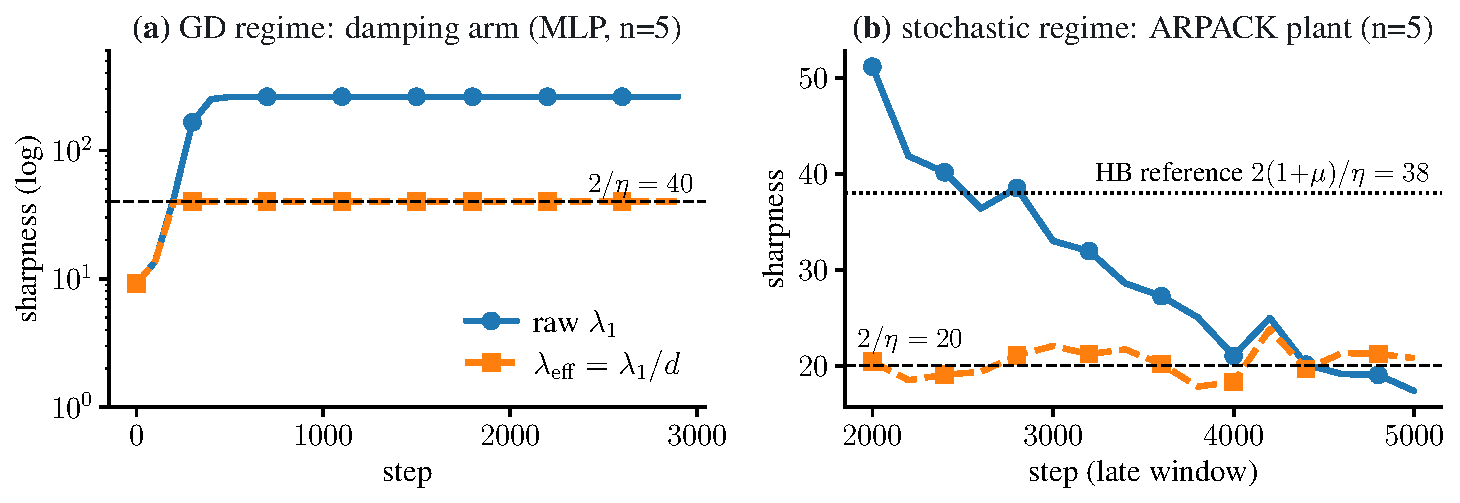
\includegraphics[width=0.95\linewidth]{34_precond_sharpness.pdf}
\caption{Control-law bookkeeping of the preconditioned sharpness
$\lambda_{\mathrm{eff}}$ (Corollary~\ref{cor:upward}) under the \emph{adaptive}
self-gating rule. \textbf{(a)} GD regime (MLP, accurate rank-1 damping,
$n{=}5$, seed-mean): the raw sensed $\hat\lambda_{1}$ escapes past
$2/\eta{=}40$ to ${\sim}\!262{\approx}6.6\cdot 2/\eta$ while
$\hat\lambda_{1}/d$ sits at $2/\eta$ throughout the climb (log scale).
This panel is \emph{definitional} whenever the clamp fires
($d=\hat\lambda_{1}/(2/\eta)$ by construction): it verifies the
control law's internal consistency, and the interventional test of the
$\lambda_{\mathrm{eff}}$ claim is the fixed-divisor control of
Fig.~\ref{fig:etad}. \textbf{(b)} Stochastic regime
(ResNet-18/CIFAR-100, accurate ARPACK-sensing damping arm, $n{=}5$,
late window): raw $\lambda_{1}$ (independent tol-$10^{-6}$ outcome
ARPACK; no statistically resolved difference from SGD) while $\lambda_{1}/d$ sits at
$20.40\pm0.65=(1.02\pm0.03)\cdot 2/\eta$, here a measurement-consistency
statement (independent outcome vs.\ stale sensing), not an identity; the
heavy-ball reference line at $38$ and the SGD raw level $29.2$ are shown for
contrast.}
\label{fig:precond}
\end{figure}

\begin{corollary}[rank-1 amplification descends below the threshold (sign-flip control)]
\label{cor:amplify}
Run the same fixed-point algebra of
the algebraic part of the restatement below at the opposite sign of the
edit: $\gamma=-\alpha<0$ (i.e.\ $g'=g+\alpha(g^{\top}u_{1})u_{1}$,
$\alpha>0$), with \textbf{A1}--\textbf{A3} otherwise unchanged. Every
sign-flip period-2 fixed point then satisfies
$y^{*}=\tfrac{2\gamma}{(1-\gamma)\eta}=-\tfrac{2\alpha}{(1+\alpha)\eta}<0$,
i.e.\ $S_{*}=2d/\eta$ with $d=\tfrac{1}{1+\alpha}\in(0,1)$:
\emph{$\lambda^{*}=2/((1+\alpha)\eta)<2/\eta$, and
$S_{*}\downarrow0$ monotonically as $\alpha\uparrow\infty$} (never below
$0$). The conditional $y$-contraction part of the restatement below becomes
$|\mu_{y}|<1$ iff $(1+\alpha)\eta^{2}\alpha_{\mathrm{ps}}<1$, \emph{harder} to satisfy as
$\alpha$ grows, unlike damping, where $\gamma\uparrow1$ makes it easier.
\emph{Experimentally confirmed} (\S\ref{sub:amp}): rank-1 amplification with
accurate warm-started sensing descends below the threshold at every tested $\alpha$, with
late-window equilibria monotone in $\alpha$, while the same sensing with
$\gamma>0$ escapes past $2/\eta$
(Lemma~\ref{prop:boundary}); the realized equilibria sit
below the naive $\lambda^{*}=2/((1{+}\alpha)\eta)$ values, consistent with
Corollary~\ref{cor:upward}'s direction-only disclaimer. (At ResNet-18
scale, rank-1 amplification shows no statistically resolved effect,
whereas increasing the amplified rank to $k{=}20$ and applying the
full-rank first-order correction both shift sharpness upward rather
than reproducing the full-batch descent
(\S\ref{sub:scale}), so the corollary's downward escape is specific
to the GD-regime dynamics.) The lemma's
negative statement is thereby \emph{sharpened, not contradicted}: what cannot
descend below the threshold is rank-1 \emph{damping} ($\gamma\in(0,1)$), not rank-1 actuation
in general.
\end{corollary}

\begin{remark}[partial multi-eigenvalue extension (separable case)]
\label{rem:separable}
If $H$ is separable, $H=\sum_{i}\lambda_{i}u_{i}u_{i}^{\top}$ with no
off-diagonal coupling, the Damian recurrence decouples into independent
$(x_{i},y_{i})$ pairs and Lemma~\ref{prop:boundary} applies
\emph{per direction}: damping any subset of eigenvectors leaves each undamped
direction's cap at $y_{i}^{*}=0$ or moves each damped direction to
$y_{i}^{*}>0$. The multi-sharp test (\S\ref{sec:control}) provides an
empirical check consistent with per-direction independence on one
non-separable landscape, the regime \citet{damian2023selfstab} leave
theoretically open. A general multi-eigenvalue extension remains open
(gap~\textbf{G1}).
\end{remark}

\paragraph{Connection to projection-based precedents.}
\citet{song2025bulk} project the SGD update onto the spectral ``bulk'' (removing
the top-$k$ eigenvector components) and report that sharpness grows unconstrained
while loss and accuracy are preserved. This is the $\gamma\!\to\!1$
($d\!\to\!\infty$) limit of our rank-1 damping: Corollary~\ref{cor:upward}'s
equilibrium $S_{*}=2d/\eta$ diverges as $d\!\to\!\infty$, so their observation
is regime~(ii) (cap removed) taken to its extreme: the unconstrained growth is
the predicted divergence of the orbit location itself, not a separate phenomenon.
Our partial-damping ($\gamma<1$) experiments diagnose the cap at finite
$S_{*}$; their full-projection ($\gamma=1$) removes it entirely. Their
``pseudo-alignment'' reading and our ``cap-removal'' reading describe the same
trajectory through different lenses; only the cap-removal lens predicts the
$\gamma$-dependent divergence quantitatively.

\begin{remark}[Connection to SAM]
\label{cor:sam}
SAM's update $\theta_{t+1}=\theta_{t}-\eta\nabla L(\theta_{t}+\rho\nabla L/\|\nabla L\|)$
does \emph{not} enter the rank-1 recurrence \eqref{eq:damped-x-formal}: expanding
to $O(\rho)$ \citep{andriushchenko2022sam}, its effective gradient is
$\nabla L^{\mathrm{SAM}}\approx(I+\tfrac{\rho}{\|g\|}H)g$, rescaling the top
direction by $1+\rho\lambda_{1}/\|g\|>1$ (curvature-amplifying), which lowers the
stability boundary SAM tracks to
$\lambda^{*}_{\mathrm{SAM}}=\tfrac{\|g\|}{2\rho}\bigl(\sqrt{1+\tfrac{8\rho}{\eta\|g\|}}-1\bigr)<2/\eta$
\citep{long2024sam}, i.e.\ $y^{*}_{\mathrm{SAM}}<0$. Rank-1 damping rescales the
top direction by $1/d<1$ (curvature-attenuating), raising the boundary to
$y^{*}>0$. This is the formal content of the attenuation-vs-amplification
dichotomy: the two edits move the EoS threshold in opposite directions
along the \emph{same} monotone $y^{*}(\gamma)$ of \eqref{eq:ystar}, and
reaching the sub-threshold region $y<0$ requires the amplifying sign. The
amplifying sign does \emph{not} have to be global: rank-1 amplification on the
top direction alone reaches $y^{*}<0$ (Corollary~\ref{cor:amplify}). At
first order, SAM contains a curvature-weighted correction whose
positive-curvature components have the amplifying sign; this motivates the
sign comparison with Corollary~\ref{cor:amplify}, but full SAM is not
identified with this linear amplification: \S\ref{sub:sammech} shows
that the finite re-query residual bundle carries the observed
endpoint difference along the tested ResNet interpolation.
\end{remark}

The assumptions above define the regime in which the reduced
recurrence is interpretable; we do not empirically certify each
assumption pointwise along every network trajectory. In particular,
spectral isolation, slow variation of the reduced coefficients, and
piecewise-constant sensing are modeling conditions rather than
measured invariants of the full network dynamics.

\paragraph{Gap inventory (2-D theorem $\to$ trajectory theorem).}
\begin{itemize}
  \item[\textbf{G1}] \emph{Multi-eigenvalue decoupling.} The lemma
        projects dynamics onto $(u_{1},\mathrm{rest})$; the multi-eigenvalue
        extension \citet{damian2023selfstab} defer (\S8.2) is open.
  \item[\textbf{G2}] \emph{Rotation singularity.} A1 fails at eigenvalue
        crossings $\lambda_{1}\leftrightarrow\lambda_{j^{*}}$, where $\nabla S$
        is singular; patching is open (empirically the trajectory crosses in
        $O(\eta^{-1})$ steps with the qualitative verdict intact).
  \item[\textbf{G3}] \emph{Time-varying $\gamma$.} A2 freezes $\gamma$; the
        extension to piecewise-constant $\gamma_{t}$ (refresh interval $N$) needs
        a perturbation analysis.
  \item[\textbf{G4}] \emph{Higher-order $x$-bounding.} Remark~\ref{rem:jacobian}'s
        fast-direction amplification is bounded by quartic-and-higher landscape
        terms the 2-D reduction omits.
  \item[\textbf{G5}] \emph{Sensing error.} A3 is ideal; with $\hat v$ at angle
        $\varphi$ to $u_{1}$ the effective damping is
        $\gamma_{\mathrm{eff}}=\gamma\cos^{2}\varphi$ and the lemma holds
        with $\gamma\to\gamma_{\mathrm{eff}}$.
\end{itemize}

\subsection{Two further controls confirm cap robustness}
\label{app:two-controls}

The lemma concerns damping the \emph{top} direction. Two further controls
test the symmetric direction and the effect of sensing lag; both confirm that
descent below the threshold did not occur for any single-direction \emph{attenuating} or
lagged edit we test (the amplifying sign is tested separately,
Corollary~\ref{cor:amplify}). The
empirical data for both live in \S\ref{sec:control} (Fig.~\ref{fig:c4lag});
here we state the structural content only.

\begin{corollary}[orthogonal damping leaves the cap intact]
\label{cor:orth}
The C4 edit $\Delta\theta=-\eta(g_{\parallel}+g_{\perp}/d)$ with
$g_{\parallel}=(g^{\top}u_{1})u_{1}$ preserves the gradient component along
$u_{1}$. Its $x$-recursion is therefore the undamped Damian map
$x_{t+1}=-(1+\eta y_{t})x_{t}$, whose period-2 fixed point is $y^{*}=0$. The
orthogonal damping rescales only the complement and does not enter the
top-direction dynamics. The cap holds for every $d$ because the $x$-recursion is the undamped Damian
map, whose sign-flip fixed point is $y^{*}=0$ \emph{regardless} of how the
$y$-drift coefficient is affected: the edit-induced correction to the drift is
odd in $x$ (zero mean per cycle) and its even remnant only renormalizes the
amplitude-setting $\beta$, which does not enter the cap location.
Experimentally confirmed in \S\ref{sec:control}
(Fig.~\ref{fig:c4lag}); the widening of per-seed variance at large $d$
reported there is a measured instance of gap~\textbf{G4}, where freezing the
complement weakens the higher-order $|x|$-bounding the 2-D reduction omits.
\end{corollary}

Together with Lemma~\ref{prop:boundary} (top-direction
damping $\Rightarrow$ $y^{*}>0$, upward escape) and Corollary~\ref{cor:orth}
(orthogonal damping $\Rightarrow$ $y^{*}=0$, cap intact), the verdict is
symmetric: damping either direction alone fails to achieve sub-threshold escape; descending
below requires the amplifying sign: global (Remark~\ref{cor:sam}) or
rank-1 local (Corollary~\ref{cor:amplify}).

\begin{observation}[short sensing lags preserve the response; the
gradient-direction proxy pins]
\label{obs:lagged}
The delayed-update sensor $\hat v_{k}=\Delta\theta_{t-k}/\|\cdot\|$ conflates
two distinct imperfections: \emph{lag}, and using the update (gradient)
direction rather than the eigenvector. Separating them shows that only the
second pins (\S\ref{sec:control}, Fig.~\ref{fig:c4lag}): the lagged-but-accurate
sensor $\hat v_{k}=\hat u(t{-}k)$ stays in regime~(ii), because $u_{1}$
rotates on the slow $O(1/\eta)$ timescale \citep{damian2023selfstab} and
$\hat u(t{-}k)\approx u_{1}(t)$ (we test only short lags $k\le3$). The lagged
update-direction sensor $\hat v_{k}=\Delta\theta_{t-k}\propto-g$, by contrast,
suffers a \emph{self-induced sensing failure}: the edit's own damping rotates
the update direction, the lagged $\hat v$ drifts off $u_{1}$, its Rayleigh
quotient collapses, the self-gating clamp sets $\gamma{=}0$, and the system
reduces to undamped Damian GD with $y^{*}=0$ (Remark~\ref{rem:regime-i}): the
operative cause is inaccuracy, not staleness.
\end{observation}
The cap is thus robust to the tested short sensing \emph{lags}
($k\le3$) but not to sensing \emph{inaccuracy}: only accurate top-direction
sensing achieves cap removal, and the failure of the delayed-update proxy is
attributable to sensing-direction inaccuracy rather than to these tested
lags.
(Without the self-gating clamp, a stale Rayleigh quotient flips $\gamma<0$ and
anti-damps to divergence: an optimizer pathology, not cap removal;
\S\ref{sec:control}.)
